\documentclass[journal]{IEEEtran}
\usepackage{amsmath,amssymb,graphicx,booktabs,array,tabularx,microtype}
\usepackage[hidelinks]{hyperref}
\renewcommand{\thesection}{S\arabic{section}}
\renewcommand{\thetable}{S\arabic{table}}
\renewcommand{\thefigure}{S\arabic{figure}}
\title{Supplementary Material\\Shielded Q-learning for Thermally-Safe, Energy-Aware Multi-Model Intrusion Detection Scheduling on Lightweight Edge Devices}
\author{Nuonan Ouyang, Adrian Shatte, Zhigang Lu, Chao Chen, and Wei Xiang}
\begin{document}\maketitle
\section{Evidence scope and chronology}
This supplement distinguishes four sources: independently held-out guard coverage, the Pi 3B+ stationary binding campaign, the corrected Pi 4B R6 online campaign, and the saved official detector test. The Pi 4B analysis contains 60 accepted cells, 36,000 windows, and 576,000 record evaluations, each window processing 16 records. These are repeated scheduler-development inputs, not 576,000 independent test samples. Per-run metrics and all paired contrasts accompany the source in \texttt{data/}; the reproduction package retains the original raw files and selection manifests.

The earlier submitted hardware-profiled replay tables cannot be numerically reproduced from their unavailable historical artifacts. Revision implementations were reconstructed and frozen. A subsequent code audit invalidated the earlier Pi 4B online campaign (V4): batch size, RiskProxy/controller behavior, masking, reward, background load, timing, and energy alignment did not consistently match the declared method. None of its policy rankings, FPR patterns, or energy results is used in the revised tables. The corrected R6 execution is a separate campaign, not relabelled V4 data.

The official detector test was opened on 11 September 2026. October corrections and corrected Q training use development inputs and validation detector-quality statistics, with no subsequent test access. The detector, preprocessor, threshold, and validation-metric hashes match those recorded at the test opening. This preserves the fixed-detector comparison but does not make the later scheduler development a fresh blinded test study. Historical output-copy provenance is incomplete; saved confusion counts can be recomputed, whereas the retained aggregates alone do not regenerate AUROC/PR-AUC.

\section{Calibration and admissibility}
Each device has fit, margin, and coverage splits of 2880 windows, spanning 72 action/batch/background cells with 40 observations per cell. Latency prediction is the fit-split 0.99 quantile in each cell. Thermal prediction uses standardized continuous features and action indicators, fitted by ordinary least squares. Residual margins use the nonnegative 0.99 quantile with the higher-order-statistic convention. A 10-ms latency buffer and $0.6^\circ$C thermal buffer are additional to the residual margins.

The Pi 3B+ held-out split has 2879 latency-covered and 2880 thermal-covered windows; its single joint miss is LUCID, n256/B2. Pi 4B has 2880 latency-covered and 2877 thermal-covered windows. Its misses occur at LUCID n1024/B1, LUCID n512/B0, and OI-SVDD+AS-ELM n64/B2, each with 39/40 covered observations in that cell. These are prediction-bound misses, not evidence of a temperature above the operating cap. No margin is tuned on these misses.

\begin{table}[t]\caption{Residual margins; the fixed buffers are added separately.}\centering\scriptsize
\begin{tabular}{llrr}\toprule
Device & Action & Latency (ms) & Thermal ($^\circ$C) \\\midrule
Pi 3B+ & FISVDD & 1.006697 & 1.001835 \\
Pi 3B+ & LUCID & 21.637906 & 1.001835 \\
Pi 3B+ & TinyDL & 0.555817 & 1.001835 \\
Pi 3B+ & OI-SVDD+AS-ELM & 1.111444 & 1.001835 \\
Pi 4B & FISVDD & 0.142454 & 1.850545 \\
Pi 4B & LUCID & 15.319520 & 1.850545 \\
Pi 4B & TinyDL & 0.345955 & 1.850545 \\
Pi 4B & OI-SVDD+AS-ELM & 0.000000 & 1.850545 \\
\bottomrule\end{tabular}\end{table}
\begin{figure}[t]\centering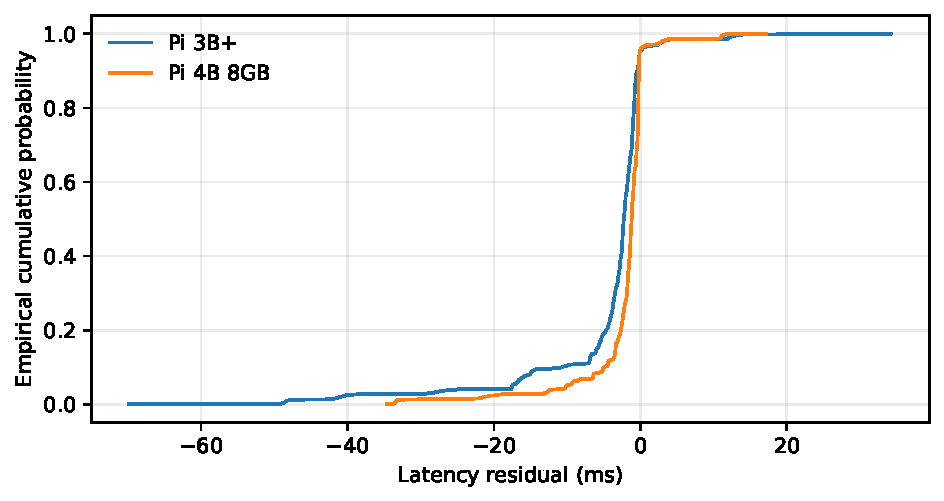
\includegraphics[width=\columnwidth]{figures/coverage_latency.pdf}
\caption{Held-out latency residual ECDFs, 2880 observations/device. The mixture covers 72 calibration cells; it is not a single-action distribution.}\end{figure}
\begin{figure}[t]\centering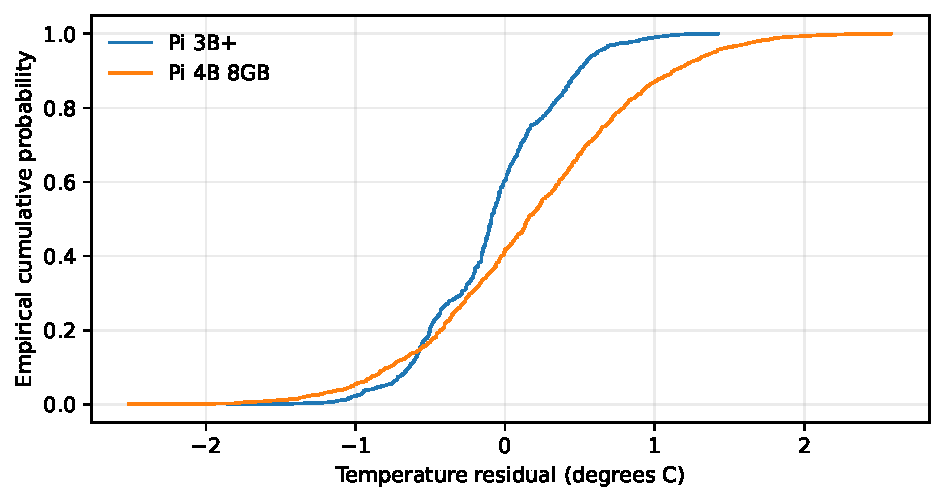
\includegraphics[width=\columnwidth]{figures/coverage_thermal.pdf}
\caption{Held-out next-temperature residual ECDFs for the same coverage splits.}\end{figure}

Runtime safety predicates use both upper predictions. The Pi 3B+ binding campaign has three admissible actions in every window; R6 Pi 4B has four. Both have zero empty-set fallbacks. Thus the unconditional admissible-action ratios are 0.75 and 1.00 with the same per-window denominators. The conditional theorem requires the prediction-error bounds; empirical quantiles alone do not guarantee them for every future state.

Stored predictor files are checked by strict SHA-256 identity. Re-fitting the archived data on a different platform is a separate numerical check: tolerance is absolute $10^{-10}$ and relative $10^{-12}$, with all held-out coverage and cap-admission Boolean decisions required to remain identical. This permits floating-point OLS differences without modifying frozen artifacts.

\section{Pi 3B+ comparison and stability}
The stationary binding campaign contains six policies, ten matched seeds, and 600 windows/run. The following aggregate is retained separately from R6; the devices and implementations are not pooled into one statistical sample.
\begin{table*}[t]
\caption{Pi 3B+ stationary binding comparison: mean $\pm$ SD across ten matched seeds; violations are total counts. Per-seed and P99 values accompany the source.}
\centering\scriptsize
\setlength{\tabcolsep}{3pt}
\begin{tabular}{lccccccr}
\toprule
Policy & F1 & FPR & Mean reward & Mean E2E (ms) & Controller (ms) & Switch cost & Viol. \\
\midrule
FSSQL-R & $0.8523\pm0.0216$ & $0.4258\pm0.0554$ & $0.5434\pm0.0338$ & $8.315\pm0.212$ & $5.903\pm0.022$ & $5.348\pm3.528$ & 0 \\
Safe-Greedy & $0.8708\pm0.0119$ & $0.3496\pm0.0404$ & $0.5839\pm0.0172$ & $7.978\pm0.023$ & $5.915\pm0.019$ & $0.000\pm0.000$ & 0 \\
Threshold & $0.8704\pm0.0120$ & $0.3508\pm0.0412$ & $0.5834\pm0.0170$ & $7.970\pm0.041$ & $5.904\pm0.031$ & $0.012\pm0.010$ & 1 \\
Unshielded-Q & $0.8523\pm0.0189$ & $0.4248\pm0.0653$ & $0.5489\pm0.0266$ & $10.114\pm1.681$ & $5.899\pm0.015$ & $4.438\pm2.629$ & 0 \\
Round-Robin & $0.8148\pm0.0136$ & $0.5737\pm0.0284$ & $0.4801\pm0.0213$ & $10.657\pm0.030$ & $5.886\pm0.023$ & $11.980\pm0.000$ & 0 \\
Static-Light & $0.7203\pm0.0193$ & $1.0000\pm0.0000$ & $0.3389\pm0.0307$ & $8.255\pm0.030$ & $5.891\pm0.020$ & $0.000\pm0.000$ & 0 \\
\bottomrule
\end{tabular}
\end{table*}


FSSQL-R minus Safe-Greedy gives mean F1 difference approximately $-0.0185$, mean reward difference $-0.0405$, and mean E2E difference $+0.3374$ ms. Exact paired sign-flip $p$ values are 0.00195 for F1, reward, and switching cost, and 0.00586 for E2E. The controller-time difference is $-0.0113$ ms ($p=0.23242$). Both policies have zero observed violations.

The single Threshold violation is seed 4109, window 111: TinyDL inference 0.446453 ms, controller 50.413877 ms, and E2E 52.521664 ms. The point latency prediction is 5.147223 ms; after residual margin and buffer the upper prediction is 15.703040 ms, leaving 24.296960 ms headroom. There is no contemporaneous switching, undervoltage, or frequency anomaly. The timings locate the long interval but do not identify an operating-system cause.

Pi 3B+ FSSQL-R rolling reward rises from 0.483742 at window 600 to 0.526027 at 6000. Mean visited states/state-actions rise from 29.7/96.3 to 34.9/118.9; greedy-policy change falls from 0.006875 to 0.000156. No window-600 Q snapshot survives, so elementwise 600-to-6000 Q drift is not reported. Sparse support and residual TD error limit the conclusion to finite-budget behavioral stability. A separate queue-transition preflight did not produce both accumulation and recovery under its frozen workload; no policy runs were executed for that extension.

\section{Corrected Pi 4B deployment}
The accepted R6 matrix is four policies by three conditions by five seeds. Two original attempts (cells 21 and 45) failed the initial temperature criterion; only their complete contemporaneous replacements enter the accepted set. The originals remain archived. These are not the V4 power-capture replacements at cells 40 and 51. The selected 60 Pi traces, meter CSVs, and run manifests are individually hash-bound.

All conditions use the same seed-specific n16 schedules. B1/B2 start a separate load process pinned to CPU 3 at 0.5/1.0 configured duty; the process is started before the ACK boundary and remains alive through the experiment. PID, affinity, configured duty, and lifecycle evidence are available. No separate utilization trace supports a claim of exactly 50\%/100\% measured CPU occupation. The queued backlog is explicitly zero; the Threshold queue input is $16+q_t$.

The complete set of 60 run summaries, all 18 condition-specific pairwise FPR contrasts, other endpoints, and the accepted-run selector are supplied as CSV/JSON files. No seed is excluded from the primary analysis. The table below reports FPR and F1 for all learned-policy seeds with the matched deterministic comparators.

\begin{table*}[t]\caption{Pi 4B per-seed outcomes and post hoc FSSQL training-support diagnostic. Static-Light FPR is 1.0 in every run.}\centering\footnotesize
\begin{tabular}{llrrrrrr}\toprule
Load & Seed & FSSQL F1 & FSSQL FPR & Greedy F1 & Greedy FPR & Threshold FPR & Unvisited states (windows) \\\midrule
B0 & 5101 & 0.9607 & 0.1358 & 0.9610 & 0.1328 & 0.1328 & 0/600 \\
B0 & 5102 & 0.9609 & 0.1302 & 0.9609 & 0.1302 & 0.1322 & 0/600 \\
B0 & 5103 & 0.9593 & 0.1399 & 0.9596 & 0.1386 & 0.1418 & 0/600 \\
B0 & 5104 & 0.9595 & 0.1377 & 0.9607 & 0.1309 & 0.1328 & 0/600 \\
B0 & 5105 & 0.9590 & 0.1453 & 0.9617 & 0.1309 & 0.1309 & 0/600 \\
B1 & 5101 & 0.9607 & 0.1358 & 0.9610 & 0.1328 & 0.1328 & 0/600 \\
B1 & 5102 & 0.9606 & 0.1315 & 0.9609 & 0.1302 & 0.1322 & 1/600 \\
B1 & 5103 & 0.9593 & 0.1399 & 0.9596 & 0.1386 & 0.1418 & 0/600 \\
B1 & 5104 & 0.9595 & 0.1377 & 0.9607 & 0.1309 & 0.1328 & 0/600 \\
B1 & 5105 & 0.9590 & 0.1453 & 0.9617 & 0.1309 & 0.1309 & 0/600 \\
B2 & 5101 & 0.8828 & 0.5425 & 0.9610 & 0.1328 & 0.1328 & 275/600 \\
B2 & 5102 & 0.8899 & 0.4940 & 0.9609 & 0.1302 & 0.1322 & 251/600 \\
B2 & 5103 & 0.8785 & 0.5637 & 0.9596 & 0.1386 & 0.1418 & 290/600 \\
B2 & 5104 & 0.9191 & 0.3414 & 0.9607 & 0.1309 & 0.1328 & 138/600 \\
B2 & 5105 & 0.8643 & 0.6579 & 0.9617 & 0.1309 & 0.1309 & 368/600 \\
\bottomrule\end{tabular}\end{table*}

The learned-policy state is reconstructed from risk, measured temperature, energy proxy, fixed backlog, and previous action. Archived training visits identify 1322 of 3000 B2 windows as states never visited in training. Their Q rows are zero and the fixed tie rule selects FISVDD. B0 and B1 have 0 and 1 such windows, respectively. This observed execution path is not a population failure rate, a proof of an attractor, or a controlled causal attribution to any one state component. It replaces, rather than supplements, the unsupported old V4 seed-5102 explanation.

\subsection{Paired inference}
The primary contrast is FSSQL-R minus Safe-Greedy within each condition. All five matched runs are retained. Percentile intervals use 2000 paired bootstrap samples with seed 20261022; exact two-sided sign-flip tests enumerate $2^5$ sign assignments. Zero-variance effect sizes are undefined, not assigned an artificial finite value. Multiple endpoints are descriptive and $p$ values are unadjusted. A positive or negative percentile interval is not substituted for an exact-test significance claim.

\begin{table*}[t]\caption{Corrected Pi 4B primary paired comparison (five matched runs per row).}\centering\footnotesize
\begin{tabular}{llrrrr}\toprule
Load & Metric & Mean difference & Bootstrap 95\% interval & Exact $p$ & $d_z$ \\\midrule
B0 & F1 & -0.00092 & [-0.00192, -0.00018] & 0.1250 & -0.834 \\
B0 & FPR & +0.00510 & [+0.00111, +0.01027] & 0.1250 & 0.879 \\
B0 & Mean reward & -0.00283 & [-0.00500, -0.00067] & 0.1250 & -0.979 \\
B0 & P99 E2E (ms) & +1.198 & [+0.242, +2.207] & 0.0625 & 0.930 \\
B0 & Energy (J) & +0.908 & [+0.173, +1.867] & 0.1250 & 0.864 \\
B1 & F1 & -0.00097 & [-0.00192, -0.00030] & 0.0625 & -0.932 \\
B1 & FPR & +0.00536 & [+0.00163, +0.01027] & 0.0625 & 0.968 \\
B1 & Mean reward & -0.00295 & [-0.00500, -0.00090] & 0.0625 & -1.067 \\
B1 & P99 E2E (ms) & +0.768 & [+0.060, +1.775] & 0.1250 & 0.689 \\
B1 & Energy (J) & -1.209 & [-1.884, -0.440] & 0.1250 & -1.392 \\
B2 & F1 & -0.07385 & [-0.08884, -0.05684] & 0.0625 & -3.615 \\
B2 & FPR & +0.38722 & [+0.29327, +0.47399] & 0.0625 & 3.356 \\
B2 & Mean reward & -0.11611 & [-0.14112, -0.08897] & 0.0625 & -3.543 \\
B2 & P99 E2E (ms) & +0.888 & [+0.152, +1.583] & 0.1250 & 0.978 \\
B2 & Energy (J) & +0.645 & [-0.874, +2.481] & 0.5625 & 0.299 \\
\bottomrule\end{tabular}\end{table*}


\begin{table*}[t]\caption{Saved official-test confusion counts and ranking metrics (82,332 rows).}\centering\footnotesize
\begin{tabular}{lrrrrrrrrrr}\toprule
Detector & TP & FP & FN & TN & Precision & Recall & F1 & FPR & AUROC & PR-AUC \\\midrule
FISVDD & 45332 & 37000 & 0 & 0 & 0.5506 & 1.0000 & 0.7102 & 1.0000 & 0.5351 & 0.6219 \\
LUCID & 45211 & 19188 & 121 & 17812 & 0.7020 & 0.9973 & 0.8240 & 0.5186 & 0.8621 & 0.8469 \\
TinyDL & 44414 & 12514 & 918 & 24486 & 0.7802 & 0.9797 & 0.8686 & 0.3382 & 0.9704 & 0.9784 \\
OI-SVDD+AS-ELM & 45218 & 15581 & 114 & 21419 & 0.7437 & 0.9975 & 0.8521 & 0.4211 & 0.9513 & 0.9584 \\\bottomrule
\end{tabular}\end{table*}

\subsection{Learning checkpoints}
The corrected Pi 4B Q tables use five development-only n16/B0 training sequences of 6000 windows, with episode resets every 600 windows. At windows 600 and 6000, mean rolling reward is 0.473583 and 0.554050, visited states are 22.2 and 25.8, and visited state-action pairs are 73.4 and 91.0. Final mean absolute TD error is 0.129277. The checkpoint change rate reaches zero, but this cannot establish behavior outside the visited state subset. Training and runtime windows are not additional independent policy replications.
\begin{figure}[t]\centering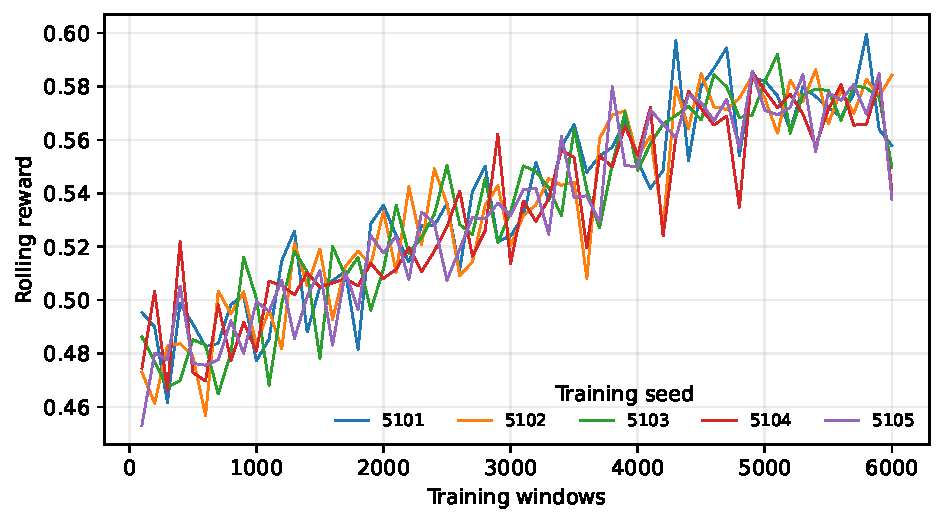
\includegraphics[width=\columnwidth]{figures/pi4b_learning.pdf}
\caption{Archived corrected Pi 4B training checkpoints for the five fixed seeds. Curves are descriptive rolling rewards, not held-out learning-performance estimates.}\end{figure}

\section{Timing and energy accounting}
The resident-model implementation measures action binding on a switch; no per-window model load is performed. Controller time begins after preprocessing and ends after binding. E2E begins at preprocessing and ends after post-action telemetry. These component intervals overlap: Q lookup is within selection, guard subcomponents are within guard, and neither should be added again to a parent total. Reward calculation, row serialization, and end-of-run label scoring are excluded from E2E and are not claimed negligible.

The KM003C trace is recorded on the Mac in a separate clock domain from Pi internal timers. The primary electrical interval is between Mac receipts of the start and end ACKs, not a comparison between unrelated Pi and Mac monotonic values. It includes scheduled idle time, background work, and tail scoring/writeout. Recorded durations are 60.070--60.282 s. Sampling is nominally 10 Hz; actual timestamps, boundary interpolation, and the trapezoidal rule are used. Integration outside the measured range is prohibited. The measurement is DC input-side and does not include AC adapter loss or the Mac.

Averaged over all conditions, controller/inference times are 4.673/0.520 ms for FSSQL-R and 4.516/0.441 ms for Safe-Greedy. The timing does not imply a measurement of all software overhead. All R6 runs have four safe actions and zero observed E2E violations. The physical energy changes sign across policy comparisons; it does not justify an energy-saving conclusion. Normalized joules per window/1000 records/correctly detected attack are in the run-level CSV. The correct-attack denominator is the run's actual TP count; it is not held-out test performance.

\section{Fixed-detector official test}
The saved test results below concern the four unchanged detectors, not online policy generalization. Thresholds are FISVDD 0.05, LUCID 0.05, TinyDL 0.315, and OI-SVDD+AS-ELM 0.065. No test-driven threshold selection is performed during the correction.

The FISVDD AUROC of 0.5351 indicates weak ranking, not merely an unfortunate binary threshold. The other detectors have stronger ranking but substantial fixed-threshold false-positive rates. We report these observations without changing the thresholds or using test outcomes in scheduler rewards.

\section{Implementation checks and availability}
The corrected worker reads the threshold configuration, executes 16 distinct inputs per window, calls the frozen RiskProxy, restricts Q argmax to admissible indices, computes the declared four reward components, and starts the configured background worker. Tests include an unsafe global-Q maximum, temperature/queue Threshold transitions, label isolation, malformed meter traces, and out-of-range integration boundaries. The accepted traces provide 16 predictions and scoring labels per window, component timing, state/action/Q evidence, background-process metadata, and bound power records. The released analysis includes FPR explicitly rather than excluding it through a field-name prefix filter.

The reproduction guide separates analysis of existing evidence from new hardware collection. Raw records, execution manifests, models, and Q tables are unchanged by this manuscript update. Historical invalid results are retained but clearly excluded. The release checksum list verifies file identity; it is not by itself a validation of algorithms or a third-party certification of measurements.
\end{document}
